\chapter{Abordare propusă, experimente, rezultate}
\label{Capitolul 5}

Pentru ca un model de inteligență artificială să învețe eficient trăsăturile necesare unei sarcini de clasificare, acesta necesită un volum mare de date de antrenare de calitate. Primul pas în dezvoltarea modelului a fost crearea unui set de date coerent, care să poată fi ulterior utilizat pentru antrenarea și testarea diverselor arhitecturi. Aceste arhitecturi sunt selectate în general pe baza performanțelor anterioare din literatură. Pentru fiecare arhitectură, s-a evaluat performanța diferitelor combinații de hiperparametri folosind metrici de performanță specifice. În urma acestor testări, a fost creată o interfață web pentru modelul cu cele mai bune rezultate, facilitând astfel utilizarea sa de către oricine. 

\section{Crearea setului de date}

Setul de date este compus din 24668 de imagini ce conțin fețe din bazele de date \textbf{Celeb-DF}\cite{li2020celeb} și \textbf{FaceForensics++} \cite{rössler2019faceforensics}. Imaginile reprezintă cadre selectate aleator din zona de mijloc a videoclipurilor pentru a asigura prezența unei fețe în prim-plan. Acestea au fost inițial împărțite în 2 categorii: imagini pozitive(clasa imaginilor reale) și imagini negative(clasa imaginilor fabricate). Apoi, pentru antrenarea și testarea optimă a modelului distribuția datelor a fost următoarea : 

\begin{itemize}
    \item 80\% date de antrenare 
    \item 15\% date de testare
    \item 5\% date de validare(folosite pentru testare în timpul antrenării)
\end{itemize}

În plus, pentru a asigura o distribuție optimă a datelor, fiecare subset conține aproximativ 50\% imagini negative și 50\% imagini pozitive. 

O problemă posibilă a acestei abordări este o performanță crescută artificial în cazul în care imagini diferite din același videoclip ar apărea în setul de antrenare, respectiv cel de testare și validare. Împărțirea finală a setului garantează faptul că imaginile din același videoclip se află toate în același subset de date. 

\begin{figure}[h]
         \centering 
         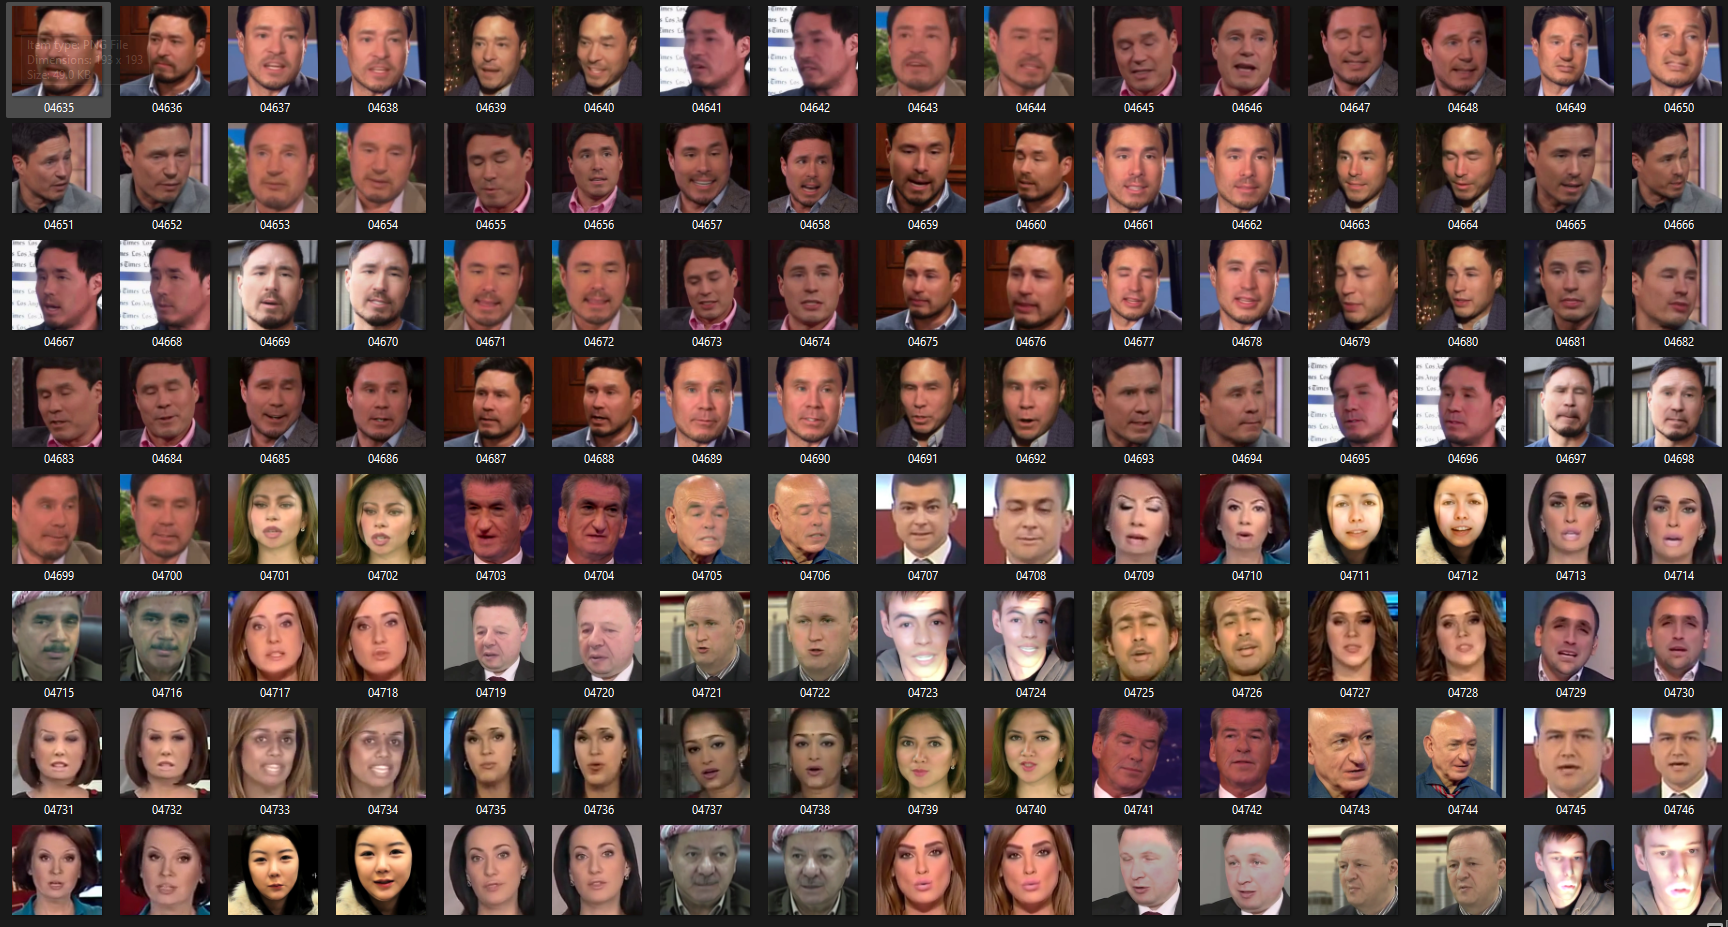
\includegraphics[width=0.75\linewidth]{images/dataset_ss.png}
         \captionsetup{font=footnotesize}
         \caption{Un director cu date extrase din videoclipuri}
\end{figure}

\subsection{Celeb-DF}

Baza de date Celeb-DF conține 5639 de videoclipuri de tip deepfake și 590 de videoclipuri reale colectate de pe platforma Youtube. Videoclipurile sunt în principal interviuri cu 59 de celebrități cu o distribuție variată a vârstei, sexului și etniei. Videoclipurile deepfake sunt obținute prin schimbarea de fețelor celor 59 de actori între ei. 

La crearea datasetului pentru modelul din lucrare au fost selectate câte 2 cadre din cele 5639 de videoclipuri deepfake și câte 10 cadre din cele 590 de videoclipuri reale. 

\newpage
\subsection{FaceForensics++}

FaceForensics++ este un set de date amplu, conceput cu scopul a facilita antrenarea modelelor de inteligență artificială pentru detectarea conținutului fabricat. Include 1000 de secvențe video originale, care au fost manipulate folosind patru metode automate de manipulare facială: Deepfakes, Face2Face, FaceSwap și NeuralTextures. Aceste videoclipuri sunt preluate din 977 videoclipuri de pe platforma YouTube, asigurând că fiecare conține o imagine frontală a feței, permițând astfel o manipulare realistică . Videoclipurile sunt disponibile comprimate în format h264 cu factori diferiți de compresie: raw, c23 și c40.

Pentru setul de date din această lucrare au fost alese videoclipurile cu compresie de tip c23. Ca și contribuție la imaginile negative au fost folosite câte 100 de materiale video generate cu Deepfakes, Face2Face, FaceSwap, respectiv NeuralTextures, din care s-au extras aleator câte două cadre conținând fețe, în timp ce din videoclipurile reale s-au extras câte 10 cadre din X videoclipuri. 

\subsection{Selecția cadrelor}

Procesarea videoclipurilor pentru extragerea imaginilor a fost realizată cu ajutorul librariilor \href{https://opencv.org/}{open-cv} și \href{https://docs.python.org/3/library/shutil.html}{shutil}. Clasa cv2.VideoCapture din OpenCV permite capturarea video prin inițializarea unui obiect de captură, citirea cadrelor și afișarea acestora. Obiectul de captură folosește un cap de citire în interiorul videoclipului, care este folosit pentru a trece de la un cadru la altul. 

Mecanismul prin care sunt alese cadrele este unul cu elemente aleatoare și poate fi descris astfel: pentru fiecare videoclip se determină numărul de cadre, iar acest număr de cadre este împărțit într-un număr arbitrar intervale egale; selecția cadrelor se face aleator din intervalul format de reuniunea intervalelor de mijloc. După o selecție, cadrul este eliminat din mulțimea de extragere pentru a nu putea fi ales de două ori. 

\begin{figure}[h]
         \centering 
         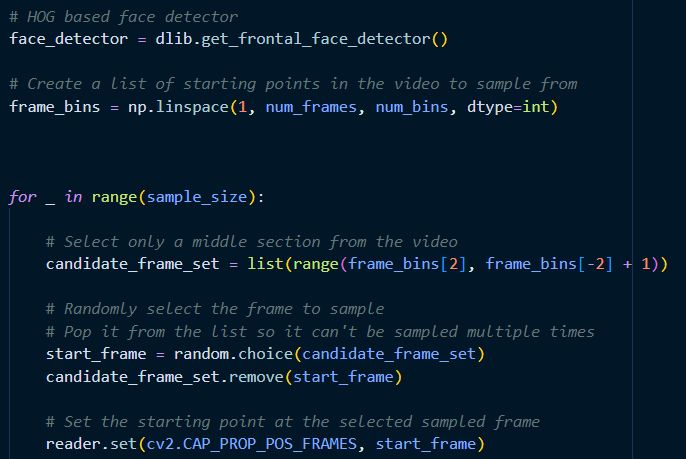
\includegraphics[width=0.65\linewidth]{images/frame_selection_ss.png}
         \captionsetup{font=footnotesize}
         \caption{Algoritmul de selecție al cadrelor}
\end{figure}

\newpage

\subsection{Extragerea fețelor}

Pentru a concentra toată puterea de învățare a modelului asupra înfățișării protagonistului, cadrele în care apar actorii nu sunt suficiente. De aceea, a fost necesară extragerea fețelor actorilor principali, lucru ce s-a realizat cu ajutorul unei funcții din modulul dlib, mai exact \texttt{get\_frontal\_face\_detector()}. 
Funcția folosește un model de inteligență artificială pre-antrenat, detecția fețelor fiind realizată cu ajutorul histogramelor de gradienți(HOG) introduse în literatură de către Navneet Dalal și Bill Trigg în 2005\cite{dalal2005histograms}.

\begin{figure}[ht]
         \centering 
         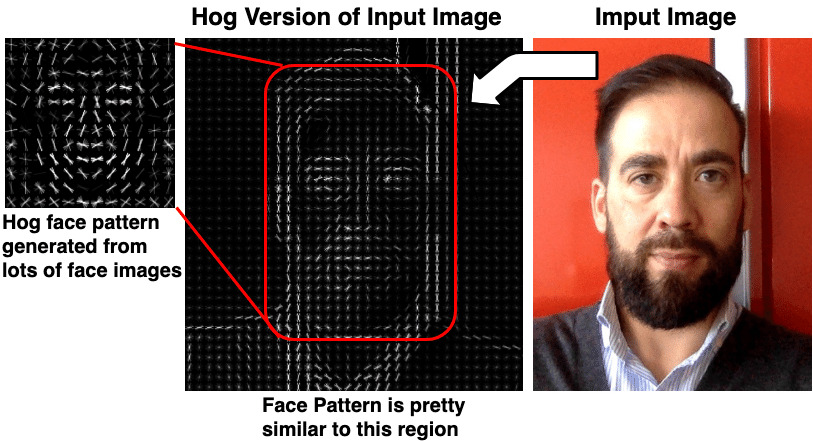
\includegraphics[width=0.75\linewidth]{images/HOG.jpg}
         \captionsetup{font=footnotesize}
     \caption{Histograme de gradienți(HOG)\cite{variz_2024}}
\end{figure}

\newpage

Histogramele de gradienți funcționează doar pentru imagini cu un singur canal de culoare, adică în tonuri de gri. Fiecare cadru extras din videoclipuri este convertit corespunzător, iar mai apoi este folosit ca parametru pentru funcția ce folosește modelul. 

\begin{figure}[ht]
         \centering 
         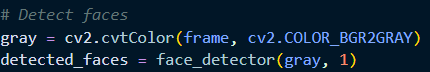
\includegraphics[width=0.8\linewidth]{images/extract_faces_ss.png}
         \captionsetup{font=footnotesize}
     \caption{Descriptorii HOG sunt folosiți pe imagini gri} 
\end{figure}

Detectorul facial folosește imaginea în tonuri de gri pentru a determina coordonatele patrulaterului ce încadrează fața detectată. Acesta returnează valorile pixelilor ce descriu fața din imagine, care mai apoi sunt folosite pentru a decupa imaginea principală și a extrage fața. 

\begin{figure}[htbp]
    \centering
    \begin{minipage}[b]{0.45\textwidth}
        \centering
        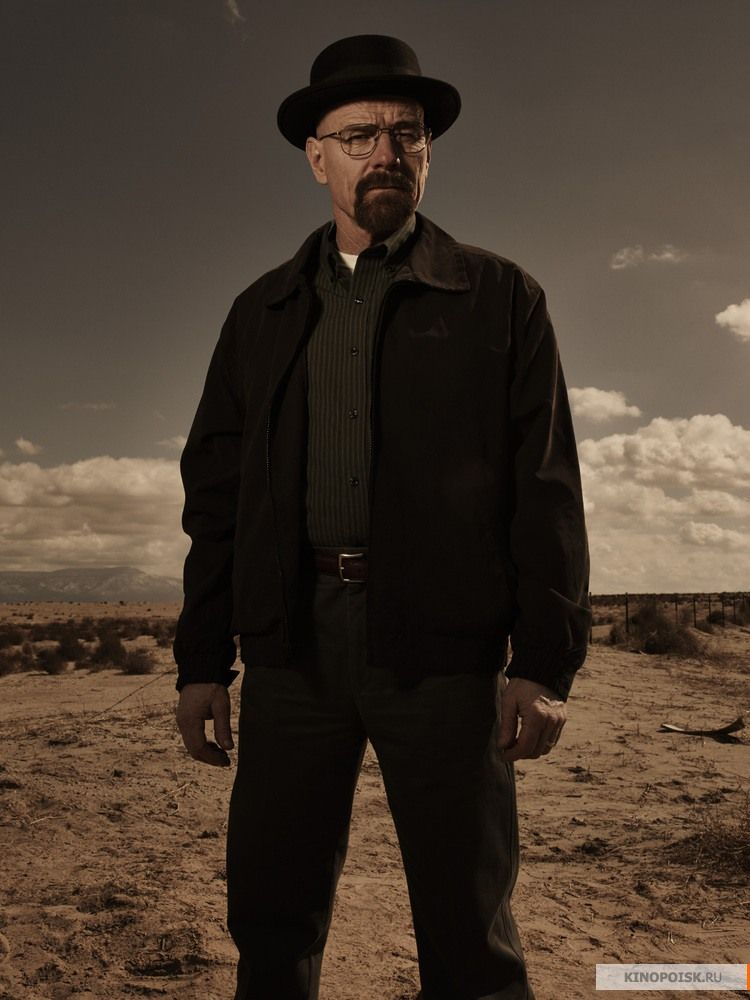
\includegraphics[width=\textwidth]{images/WW.jpg}
        \caption{Imaginea originală}
    \end{minipage}
    \hfill
    \begin{minipage}[b]{0.45\textwidth}
        \centering
        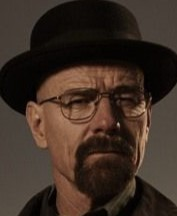
\includegraphics[width=\textwidth]{images/WW_face.jpg}
        \caption{Fața decupată din imagine}
    \end{minipage}
\end{figure}

\section{Selecția arhitecturilor}

Având la dispoziție setul de date creat, următorul pas a fost selectarea unui model de inteligență artificială care se pliază pe scopul aplicației finale și în același timp să aiba un număr de parametri proporțional cu puterea de calcul a sistemului folosit. 

Când vine vorba de sarcini ce includ utilizarea de imagini, arhitecturile convoluționale și, mai nou, cele de tip vision transformer, sunt opțiunile cele mai performante. Pentru ca timpul de antrenare și testare să fie fezabil, pentru această aplicație decizia a fost ca modelul ales să fie o rețea neuronală convoluțională. 

Un alt aspect important al antrenării modelelor de inteligență artificială este utilizarea de modele pre-antrenate pe alte seturi de date ca punct de plecare pentru învățarea unui set de date. Acest proces se numește \textbf{transfer learning}. Este des întâlnit în literatură deoarece s-a dovedit a fi foarte eficient și utilizarea acestui procedeu este facilitată de disponibiliatea în framework-urile de învățare automată a mai multor modele pre-antrenate des folosite. 

\subsection{ResNet}

ResNet este o arhitectură convoluțională introdusă de către Kaiming He et al. în anul 2016\cite{he2016deep} și a reprezentat o revelație în vederea artificială, câștigând detașat competiția ImageNet. 

ResNet este considerată o arhitectură puternică datorită mai multor caracteristici inovatoare și avantaje pe care le oferă. Una dintre principalele inovații aduse de ResNet este utilizarea blocurilor reziduale. Aceste blocuri permit antrenarea rețelelor neuronale foarte adânci fără a suferi de problema gradienților care dispar(vanishing gradients), o problemă comună în rețelele adânci care face ca gradienții să devină foarte mici, îngreunând astfel antrenarea eficientă.

Blocurile reziduale folosesc o conexiune directă (skip connection) între straturi, ceea ce permite ca informația să fie transmisă direct peste mai multe straturi. Acest lucru ajută modelul să păstreze informațiile esențiale și să învețe mai eficient caracteristicile relevante ale datelor. 

\begin{figure}[ht]
         \centering 
         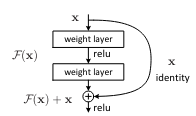
\includegraphics[width=0.3\linewidth]{images/bloc_rezidual.png}
         \captionsetup{font=footnotesize}
     \caption{Bloc rezidual\cite{he2016deep}} 
\end{figure}

ResNet este, de asemenea, flexibilă și scalabilă. Arhitectura sa permite construirea unor rețele foarte adânci, cum ar fi ResNet-50, ResNet-101 sau chiar mai adânci, fără a compromite performanța. Această adâncime suplimentară permite modelului să capteze și să învețe caracteristici extrem de complexe și detaliate din datele de antrenament.

Pentru setul de date disponibil, arhitectura aleasă a fost ResNet-50, un model cu 25M(25 de milioane) de parametri, având și un model pre-antrenat pe setul de date ImageNet, disponibil în \href{https://pytorch.org/vision/master/models/generated/torchvision.models.resnet50.html#torchvision.models.resnet50}{PyTorch}. 

\subsection{EfficientNet}

Modelul EffcientNet a fost propus de către Mingxing Tan și Quoc V. Le în anul 2019 \cite{tan2019efficientnet} printr-o lucrare care avea ca scop oferirea unei analize și al unui mod eficient de a scala rețelele neuronale convoluționale  Aceasta se realizează prin ajustarea simultană a dimensiunilor de adâncime, lățime și rezoluție a rețelei într-un mod coordonat și echilibrat. Spre deosebire de metodele tradiționale care măresc doar una dintre aceste dimensiuni, abordarea EfficientNet optimizează utilizarea resurselor și îmbunătățește performanța generală.

\begin{figure}[ht]
         \centering 
         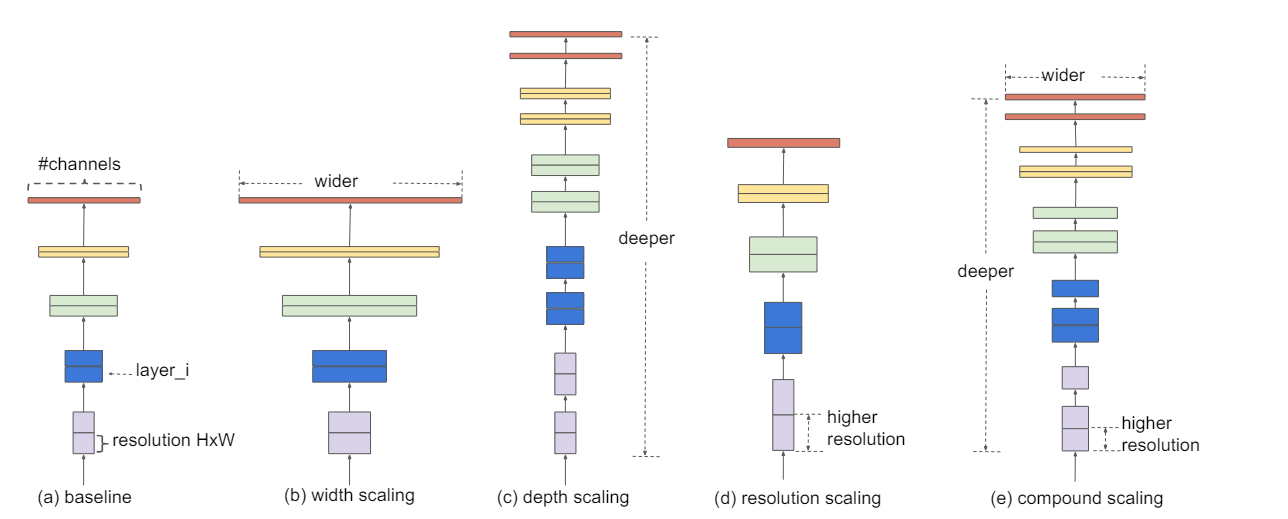
\includegraphics[width=0.7\linewidth]{images/effnet_arch.png}
         \captionsetup{font=footnotesize}
     \caption{EfficientNet foloște o scalare eficientă a rețelei\cite{tan2019efficientnet}} 
\end{figure}

\newpage

Arhitectura este, de asemenea, foarte eficientă din punct de vedere computațional. Datorită designului său optimizat EfficientNet este capabilă de performanță folosind mai puține resurse computaționale față de alte modele mai adânci. Acest lucru face ca EfficientNet să fie o alegere excelentă pentru aplicații unde resursele de calcul sunt limitate. 

\subsection{RegNet}

RegNet este o arhitectură dezvoltată cu scopul de a fi antrenată într-un mod eficient și scalabil. Modelul a fost introdus de către departamentul de inteligență artificială de la Facebook(FAIR)\cite{radosavovic2020designing} și se remarcă prin simplitatea și performanțele sale. RegNet reușește sa aibă rezultate competitive cu alte arhitecturi, fiind mult mai simplă de implementat și înțeles. 

Arhitectura este compusă din mai multe etape, fiecare conținând o serie de blocuri. Această abordare pe etape permite rețelei să crească treptat în adâncime și complexitate. În cadrul acestor etape, RegNet folosește blocuri de tip bottleneck, similare cu cele utilizate în arhitecturile ResNet, care ajută la menținerea eficienței computaționale pe măsură ce adâncimea rețelei crește.

% \begin{figure}[ht]
%          \centering 
%          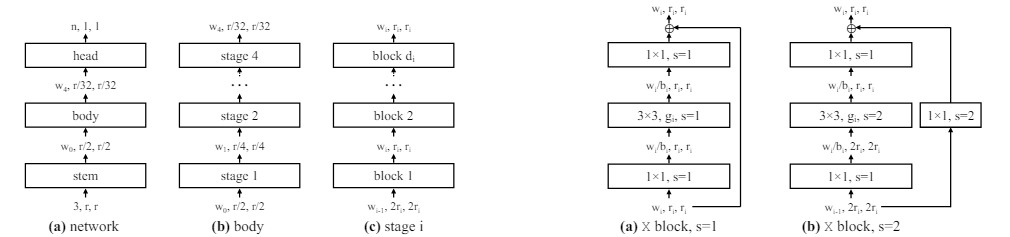
\includegraphics[width=\linewidth]{images/regnet.png}
%          \captionsetup{font=footnotesize}
%      \caption{Structura pe etape și blocuri a arhitecturii RegNet\cite{radosavovic2020designing}} 
% \end{figure}

O caracteristică ce scoate în evidență arhitectura este utilizarea spațiilor de design, introduse ca noutate în lucrare, un concept care permite explorarea și optimizarea diferitelor configurații de rețea. Prin utilizarea de diverși parametri, cum ar fi numărul de canale (lățimea) și numărul de straturi (adâncimea), cei care proiectează rețeaua pot identifica cele mai eficiente modele fără să mai treacă prin încercări repetate.

În ceea ce privește performanța, modelele RegNet au rezultate competitive pe setul de date ImageNet, capabile să concureze cu arhitecturi mai complexe. În plus, design-ul RegNet asigură eficiență computațională, ceea ce îl face folositor pentru dezvoltarea de modele capabile cu resurse limitate.



\section{Experimente și rezultate}
\label{SubCh: experimente și rezultate}
\section{Creșterea performanței cu ajutorul Test Time Augumentation(TTA)}
